\documentclass{article} % For LaTeX2e
\usepackage{nips13submit_e,times}
\usepackage{hyperref}
\usepackage{url}
\usepackage{enumitem}
\usepackage[]{algorithm2e}
\usepackage{amsmath}
\usepackage{graphicx}
\usepackage{caption}
\usepackage{subcaption}
\usepackage{float}
\captionsetup[algorithm]{labelfont=rm,labelsep=period}

%\documentstyle[nips13submit_09,times,art10]{article} % For LaTeX 2.09


\title{Movie Recommendation based on Collaborative Topic Modeling}


\author{
Abhishek Bhowmick \\
Department of Computer Science\\
Carnegie Mellon University\\
Pittsburgh, PA 15213 \\
\texttt{abhowmi1@andrew.cmu.edu} \\
\And
Udbhav Prasad \\
Department of Computer Science\\
Carnegie Mellon University\\
Pittsburgh, PA 15213 \\
\texttt{udbhavp@andrew.cmu.edu} \\
\And
Satwik Kottur \\
Department of Electrical Engineering\\
Carnegie Mellon University\\
Pittsburgh, PA 15213 \\
\texttt{skottur@andrew.cmu.edu} \\
}

% The \author macro works with any number of authors. There are two commands
% used to separate the names and addresses of multiple authors: \And and \AND.
%
% Using \And between authors leaves it to \LaTeX{} to determine where to break
% the lines. Using \AND forces a linebreak at that point. So, if \LaTeX{}
% puts 3 of 4 authors names on the first line, and the last on the second
% line, try using \AND instead of \And before the third author name.

\newcommand{\fix}{\marginpar{FIX}}
\newcommand{\new}{\marginpar{NEW}}

%\nipsfinalcopy % Uncomment for camera-ready version

\begin{document}

\maketitle

\begin{abstract}
Traditional collaborative filtering relies on reviews provided by viewers
in the movie watching community to make recommendations to the user. In this
project, we attempt to combine this approach with probabilistic topic modeling
techniques to make recommendations that consist not only of movies that are
popular in the community, but also those that are similar in content to movies
that the user has enjoyed in the past.  
\end{abstract}

\section{Introduction}

Recommender systems are an important technology for TV/movie streaming
services like Netflix, HBO, audio/music streaming sites like Spotify, 
Pandora, news article feeds like Pulse, online retailers such as Amazon, Walmart
etc. Indeed, any service provider or content management system that has large
quantities of information (or the ability to extract such information) such as 
usage patterns, browsing and click history, natural text descriptions etc can
and should make use of recommendation methods to help find items of interest. 
Among various information sources, data in the form of natural text is a 
particularly rich and expressive source of information, however it is highly 
unstructured in general. Topic models are used to extract latent structures
from large volumes of unlabeled text, that can be used for analysis of 
contents and in turn, aid end goals such as making recommendations. In
particular, textual information such as movie plot summaries can be very
helpful to improve the prediction performance of traditional movie
recommendation based on collaborative filtering. In the remaining 
part of this report, we limit ourselves to the study of how topic modeling of 
large text corpora can help in the task of movie recommendation, however most 
of the discussion/analysis can be applied to other domains.  

\subsection{Collaborative Filtering and its shortcoming}

Traditional collaborative filtering makes use of interactions between users and 
items. They may be broadly classified into two categories - neighbourhood methods and latent factor models. Neighbourhood models explicitly capture relationships between items (or users) and predict a user's liking for a particular item based on ratings of neighbouring items by the same user. The other approach, latent
factor models, directly characterize both users and items by latent factors. We focus on factor based models as they are more accurate than neighbourhood based 
methods. However, all collaborative filtering methods suffer from the `cold 
start' problem, that is 
they are unable to recommend movies in the absence of rating patterns. In fact, 
in the domain of music, it has been observed \cite{music-long-tail} that the distribution of available rating information for music artists has a very long tail, meaning that most of the music items have little rating data available. We believe the same is true of movies as well and hence, would like to be able to recommend movies that are in this long tail. 


%Traditional collaborative filtering techniques make use of usage patterns, 
%or more specifically, movie reviews. Movie ratings provided by a user
%are used alongwith similar ratings by other users to build a model that captues the user's preferences. This model is then used to predict movies that the user
%may have an interest in. However, this method only works when sufficient usage
%data is available. New content that is available may not be possible to recommend in absence of sufficient usage data. This is known as the 'cold start' 
%problem.
%
%One strategy might be to randomly recommend newly arrived movies to users and record their responses, thus building up usage data. However, such an approach has
%a few shortcomings. Since an average user likes only a few types of movies, it 
%is more likely than not for the user to give a negative review to a randomly suggested movie. Getting a sufficient number of positive reviews may take a long
%time through this approach, and also user satisfaction decreases due to the 
%bad recommendations made by the system (assuming a random recommendation is more
%likely to be bad than good). 


\subsection{Content Based Recommendation}

Content-based recommendation addresses the `cold start' problem associated with 
collaborative filtering, where certain items do not have any rating information 
and hence the corresponding item vectors consist of all zeroes (we use 
zeroes to represent missing ratings in the rating matrix). One approach is to 
use topic modeling on movie plot summaries to identify latent themes/topics. We 
can learn topic representations for each item (a vector of topic proportions) 
and add them to the item vectors in the latent-factor model. Such topic 
representations of movie items are also useful outside the domain
of movie recommendation. Interpretability of topics may help in explaining 
recommendations to users, effective content programming and ad targeting based
on user profiles \cite{fLDA}. 
 
%A simple way is to make
%recommendations based on movie metadata such as genre, actors, language etc. 
%However, this approach severely restricts the pool of movies from which new 
%recommendations can be made. It also leads to very predictable results, 
%since recommendations made on the basis of metadata alone resemble the results
%a user would have got through simple keyword searches.

%gA much more interesting approach is to identify similarities among movies 
%gthrough latent themes extracted from information such as plot summaries. Topic 
%gmodeling can be used to describe movies in terms of such latent themes. Such an
%gapproach can allow the recommendation system to generalize to new movies that 
%ghave very little usage data.

\section{Problem Definition}

Briefly, the problem we are trying to solve is predict how highly a user will 
rate certain movies based on all users' rating histories and plot summaries for 
all movies. Making use of these predicted ratings, we come up with movie 
recommendations for a user. The problem can be formalized as follows 
\cite{grouplens} :

We are given a list of users \textit{U} = $\{u_{1}, u_{2} ... u_{m}\}$ and a 
list of items \textit{V} = $\{v_{1}, v_{2} ... v_{n}\}$, where each user $u_{i}$
has a list of items $I_{u_{i}}$ which he/she has given ratings for. For a given
user $u_{a} \in \textit{U}$, we need to solve the following two tasks:

\begin{itemize}[leftmargin=*]

\item[] {\bf Prediction}: Estimate the predicted rating $P_{a_{j}}$ of an
item $v_{j} \notin V_{u_{a}}$. The prediction task can be further split into
two types: \textit{in-matrix prediciton} and \textit{out-of-matrix prediction}. 
\textit{In-matrix prediction} is the problem of predicting ratings for items
that have already been rated by atleast twenty other users, whereas 
\textit{out-of-matrix prediction} makes predictions about those items that have
very few or no ratings (less than 20).

\item[] {\bf Recommendation}: Return a list of N items $I_{r} \in I \:\&\: I_{r} \cap I_{a} = \phi$, that the user will like most. This is simply a problem of
returning the items with highest predicted rating values.

\end{itemize}

Specifically, we are interested in observing how incorporation of item topic 
representations increases the prediction accuracy of factor models. We would
also like to analyse the interpretability of the latent topics that are 
captured by the topic model, however this will be just be a qualitative 
analysis.

\section{Proposed Method}
\label{gen_inst}

We use Probabilistic Matrix Factorization (PMF) for collaborative filtering on 
movie ratings and Latent Dirichlet Allocation (LDA) for topic modeling of the 
corpus of movie plot summaries. We then combine the latent factor model learned
through PMF and the topic model learned through LDA into a single
collaborative topic regression model (CTR). A CTR model essentially uses the
latent topic space (latent variables) to explain observed ratings and observed 
documents (observed variables), thus incorporating content information into a 
collaborative filtering framework \cite{ctr}.

\subsection{Probabilistic Matrix Factorization}


\subsection{Latent Dirichlet Allocation}
For a collection of text documents, a topic modeling algorithm extracts a set of
`topics', where each `topic' is a distribution over words that occur in the
documents. Words belonging to a topic are biased around a single theme. The
topic model that we use for representation of documents is Latent Dirichlet 
Allocation (LDA), which is a
generative probabilistic graphical model for collections of discrete data \cite{lda}. Each document in the corpus is modeled as a finite mixture over a set of 
underlying topics.

%The tf-idf scheme \cite{tf-idf} reduces each document in a corpus to a vector 
%of real numbers,
%each of which represents a ratio of `term frequency' count to an `inverse 
%document frequency' count (suitable normalized). However, this representation
%is extremely high dimensional and captures very little intra and inter document
%statistical structure. Latent Semantic Indexing (LSI) \cite{lsi} reduces the 
%high dimensionality of the tf-idf term-document matrix through a singular value 
%decomposition. However, this technique was replaced by a generative
%probabilistic model which is the pLSI model (probabilistic LSI) \cite{}.  

LDA has the underlying assumptions that the words in a document and documents
in a corpus are exchangeable - i.e., the specific ordering of words and
documents can be neglected. Now, De Finetti's representation theorem states that
a collection of infinitely exhangeable random variables are conditionally 
independent and identically distributed, if they are conditioned on a random
parameter that is drawn from some probability distribution. Now, the generative
process of the LDA model is:

\begin{algorithm}
initialize vocabulary from corpus, the size of which is V\;
\For{each of the K topics k}{
	Choose $\beta_{k,1:V}$ $\sim$ Exhangeable Dirichlet($\eta$) // Draw topic distributions\; 
}
\For{each of the M documents {\bf w} in corpus D}{
Choose $\theta$ $\sim$ Dirichlet($\alpha$)\;
	\For{each of the N words $w_{n}$ in document {\bf w}}{
	Choose a topic $z_{n}$ $\sim$ Multinomial($\theta$)\;
	Choose word $w_{n}$ from $p(w_{n} | z_{n}, \beta_{z_{n}})$, a multinomial
	probability conditioned on topic $z_{n}$
	}
}
\caption{Generative process for LDA}
\end{algorithm}

\begin{figure}[h]
	\centering
	\captionsetup[subfigure]{oneside,margin={0cm,1.8cm}}
	\begin{subfigure}[b]{0.45\textwidth}
	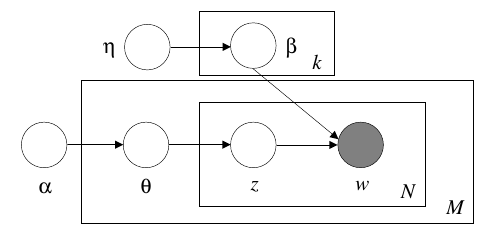
\includegraphics[width=6cm,height=6cm,keepaspectratio]{lda-model.png}
	\caption{True posterior distribution}
	\label{fig:lda-model}
	\end{subfigure}
	~
	\begin{subfigure}[b]{0.5\textwidth}
	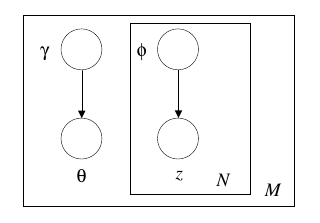
\includegraphics[width=8cm,height=3cm,keepaspectratio]{lda-variational.png}
	\caption{Variational posterior distribution}
	\label{fig:lda-variational}
	\end{subfigure}
\caption{Graphical models of LDA, before and after variational approximation}
\label{fig:models}
\end{figure}


Figure~\ref{fig:lda-model} shows the graphical model representation of LDA, which is
a three-level hierarchical model. We
assume that the number of topic vectors k is fixed and the vocabulary size of
the corpus to be modeled is V. Now, the word probabilities are parametrized
by a k X V random matrix $\beta$, each row of which represents the distribution 
of topics over words in the vocabulary. Each row of $\beta$ is independently 
drawn from an exchangeable Dirichlet distribution with parameter $\eta$.
Also, $\alpha$ is a k-dimensional vector 
which is a parameter for the Dirichlet random variable $\theta$. Given the
parameters $\alpha$ and $\beta$ (which itself is a random matrix parametrized
by $\eta$), the joint distribution of the topic mixture
$\theta$, the set of N topics {\bf z} and the set of N words {\bf w} is:

\begin{equation} \label{eq1}
p(\theta,{\bf w},{\bf z} | \alpha,\beta ) = p(\theta|\alpha)\prod_{n=1}^{N}p(z_{n}|\theta)p(w_{n}|z_{n},\beta) 
\end{equation}

We make use of the representation theorem which states that the set of topics
{\bf z} are independent conditioned on $\theta$ which is a random parameter of 
a multinomial distribution. Next, we describe two important tasks for LDA, 
namely inference and estimation:

\begin{itemize}[leftmargin=*]

\item[] {\bf Inference}: The inference task is to compute the posterior 
distribution of the hidden variables given the observed variable {\bf w} (the 
document), assuming we know the parameters $\alpha$ and $\beta$. (Note that 
we treat $\beta$ as a fixed parameter for the following discussion)

\begin{equation} \label{eq2}
p(\theta,{\bf z} | {\bf w},\alpha,\beta ) = \frac{p(\theta,{\bf z}, {\bf w}|\alpha,\beta)}{p({\bf w}|\alpha,\beta)} 
\end{equation}

Computing this distribution is intractible and hence we use variational 
approximate inference, as described by Blei et al. \cite{lda}. Simple 
modifications to the LDA graphical model such as dropping edges between 
$\theta$, {\bf z} and 
{\bf w} and adding variational parameters lead us to the variational model as inFigure~\ref{fig:lda-variational}, which has the following variational distribution:
 
\begin{equation} \label{eq3}
q(\theta,{\bf z}|\gamma, \phi) = q(\theta|\gamma)\prod_{n=1}^{N}q(z_{n}|\phi_{n})
\end{equation}

The optimal values of the variational parameters ($\gamma^{*}$, $\phi^{*}$) are 
obtained by minimizing the
Kullback-Leibler (KL) divergence between the variational and true posterior
distribution. By placing a Dirichlet prior on $\beta$, we get a separable 
variational distribution, which yields the same expressions for $\gamma^{*}$, 
$\phi^{*}$ and introduces a new variational parameter $\lambda$ which has a 
similar expression as $\gamma$.

\item[] {\bf Estimation}: We wish to find parameters $\alpha$ and $\eta$ that
maximize the log-likelihood of observed data, however computing the likelihood
is intractable. So, we use a variational EM procedure in which we alternatingly
maximize a lower bound on the log-likelihood of data with respect to 
variational parameters $\gamma$, $\phi$ and $\lambda$. This is the E-step. We 
then maximize this lower bound with respect to the parameters $\alpha$ and 
$\eta$, which comprises the M-step. The updates for both the parameters $\alpha$
and $\eta$ are obtained using an efficient Newton-Raphson method in which 
Hessian is inverted in linear time.

\end{itemize}

\subsection{Collaborative Topic Regression}

The Collaborative Topic Regression (CTR) model combines a topic model such as
LDA with traditional collaborative filtering \cite{ctr}. This is done by
combining both the latent topic vector and observed ratings to describe the
item latent vector in the factor model of Section~\ref{sec:pmf}. The graphical
model and generative process of CTR are given below:

%\begin{algorithm}
%\For{each user i}{
%	Draw user latent vector $u_{i}$ $\sim$ $\mathcal{N}(0,\sigma^{2}\lambda_{u}^{-1}I_{K}$)\; 
%}
%\For{each item j}{
%	Draw topic proportions $\theta_{j}$ $\sim$ Dirichlet($\alpha$)\;
%	Draw item latent offset $\epsilon_{j}$ $\sim$ $\mathcal(N)(0, \sigma^{2}\lambda_{v}^{-1}I_{K})$\;
%	Set item latent vector as $v_{j} = \epsilon_{j} + \theta_{j}$\;
%	\For{each word $w_{jn}$}{
%		Draw a topic assignment $z_{jn}$ $\sim$ Multinomial($\theta$)\;
%		Draw word $w_{jn}$ $\sim$ Multinomial($\beta_{z_{jn}}$)\;
%	}
%}
%\For{each user-item pair (i,j)}{
%	Draw the rating $r_{ij}$ $\sim$ $\mathcal{N}(u_{i}^{T}v_{j}, \sigma^{2}I)$\;
%}
%\end{algorithm}
\begin{figure}[h]
	\centering
	\captionsetup[subfigure]{oneside,margin={0cm,1.8cm}}
	\begin{subfigure}[b]{0.45\textwidth}
	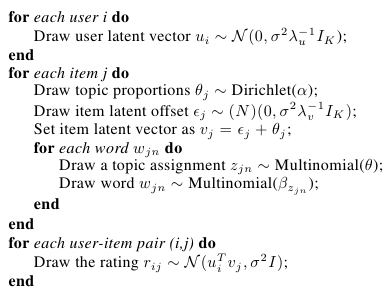
\includegraphics[width=6cm,height=6cm,keepaspectratio]{ctr-gen-process.png}
	\caption{Generative process of CTR}
	\label{fig:ctr-gen}
	\end{subfigure}
	~
	\begin{subfigure}[b]{0.45\textwidth}
	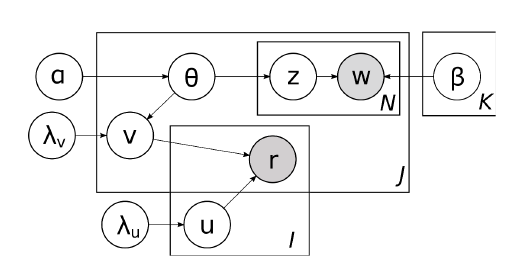
\includegraphics[width=6cm,height=8cm,keepaspectratio]{ctr-model.png}
	\caption{Graphical model of CTR}
	\label{fig:ctr-model}
	\end{subfigure}
\caption{Generative process and model of CTR}
\label{fig:ctr}
\end{figure} 

\begin{itemize}[leftmargin=*]

\item[] {\bf Parameter Estimation}: First, we train our LDA implementation on a separate training corpus and learn the model parameters $\alpha$ and $\beta$. 
Now, the log likelihood of the data is given by:
\begin{equation} \label{eq4}
\mathcal{L} = \frac{-\lambda_{u}}{2}\sum_{i}u_{i}^{T}u_{i} -
		\frac{\lambda_{v}}{2}\sum_{j}(v_{j}-\theta_{j})^{T}(v_{j}-\theta_{j})
		+ \sum_{j}\sum_{n}log(\sum_{k}\theta_{jk}\beta_{k,w_{jn}})
		- \sum_{i,j}\frac{1}{2\sigma^{2}}(r_{ij}-u_{i}^{T}v_{j})^{2}
\end{equation}

Computing the full posterior of $u_{i}$, $v_{j}$ and $\theta_{j}$ given
parameter $\beta$ is intractable. Our approach is to maximize the likelihood
function by co-ordinate ascent, iteratively optimizing the collaborative
filterings {$u_{i}$, $v_{j}$} and topic proportions $\theta_{j}$. Given
topic estimate $\theta_{j}$, setting the gradient of the log likelihood with 
respect to $u_{i}$ and $v_{j}$ equal to zero gives us closed form update rules
for the collaborative filtering variables. Similarly, in the next phase, we can
optimize the topic estimate $\theta_{j}$ given $u_{i}$ and $v_{j}$. However,
similar to the approach taken by Blei et al. \cite{ctr}, we simply set 
$\theta_{j}$ equal to the topic estimate obtained from our LDA implementation,
to save computation time without significant performance loss.\footnote{We 
use the movies for which we have both ratings and plot summaries to learn
the optimal parameters $u_{i=1:I}^{*}$, $v_{j=1:J}^{*}$, $\theta_{1:J}^{*}$,
$\beta^{*}$. We also use include these movies in the training corpus of our 
LDA.}

\item[] {\bf Prediction} : We then use the learned parameters for prediction
of movie ratings. For in-matrix prediction, we use the following approximation:

\begin{equation} \label{eq5}
r_{ij}^{*} \approx (u_{i}^{*})^{T}(\theta_{j}^{*}+\epsilon_{j}^{*}) = (u_{i}^{*})^{T}v_{j}^{*}
\end{equation}

For, out-of-matrix prediction, where the movie has no ratings available, we use 
the following approximation:

\begin{equation} \label{eq6}
r_{ij}^{*} \approx (u_{i}^{*})^{T}(\theta_{j}^{*})
\end{equation}

\end{itemize}


\section{Experiments}

We present the results of our evaluations and analysis in this section. We
denote the plain collaborative filtering model as CF ($v_{j}=\epsilon_{j}$), the
collaborative topic regression model as CTR ($v_{j}=\epsilon_{j}+\theta_{j}$) 
and the prediction model with just topic estimates as CTR-LDA 
($v_{j}=\theta_{j}$), where $v_{j}$, $\epsilon_{j}$ and $\theta_{j}$ are the 
latent vector, offset vector and topic estimate vector respectively for item j.

\subsection{Dataset}

For Collaborative Filtering, we use the MovieLens 10M dataset
\footnote{http://grouplens.org/datasets/movielens/}, which is a collection of 
10 million movie ratings on 10,000 movies by 72,000 users. The dataset has been 
pre-processed so that each user has rated at least 20 movies. This makes the 
rating matrix very sparse (98.6\% sparse). The data is very well structured 
and fits into memory. The range of the rating values is 1 - 5, in steps of 0.5.

We use the CMU Movie Summary Corpus\footnote{http://www.ark.cs.cmu.edu/personas/} for generative topic modeling of the movie summaries. This
corpus has plot summaries for 42,306 movies and associated metadata such as 
genre, year of release, cast etc. Each movie is indexed by a Wikipedia Movie ID.
We use only the plot summary text and none of the other metadata. 

The datasets are used in the following manner: we first find the set of movies 
for which we have both plot summaries and user ratings - this common subset has
approximately 5000 movies in total. Out of these, we choose 4400 movies and 
collect their ratings, 80\% of which we use for training our CTR and CTR-LDA 
models and 20\% for in-matrix prediction test. We use the remaining 600 movies
from the common subset for out-matrix testing of CTR and CTR-LDA. We 
separately train the topic model using nearly 37,000 movie summaries for
which we do not have any user ratings. 

Since the movie summaries are in the form of natural text, some preprocessing
steps were necessary - namely tokenizing, upper-case to lower-case conversion,
punctuation and stop-word removal and stemming. We used the python NLTK toolkit 
\cite{nltk} for this. We extracted all words from the processed summaries and 
built our vocabulary after sorting them lexicographically. Each document was 
then represented as a vector of integers, each integer being an index into the 
vocabulary. For ease of combining the summary and rating datasets, we 
created a map from the Wikipedia IDs to the Movielens IDs (by linking movie IDs 
that have the same movie names). 

\subsection{Evaluation of LDA}

We evaluate the interpretability of latent topics discovered by our LDA
implementation using two human evaluation tasks namely, {\textit word intrusion}
and {\textit topic intrusion}, proposed by Chang, Blei et al \cite{tea-leaves}. 
These tasks evaluate the quality of topics inferred by the model and the 
assignment of topics to documents. We describe these tests in more detail and
evaluate our LDA using these below:

\subsubsection{Word Intrusion}
This test measures whether the topics inferred by the topic model correspond
to natural interpretations and contain words that are semantically close. An
`intruder' is defined as a word that doesn't belong with the the others in a 
group. The original task proposed in \cite{tea-leaves} consists of 
building a set of words from a randomly chosen topic and injecting an `intruder'from some other topic. This set is then presented to a human subject to see if 
the `intruder' is correctly identified within the presented set. We modify the 
test for our evaluation. We list out some of the topics from a 15-topic 
LDA and identify the `intruders' in each topic and try to interpret themes
represented by each of these topics.

\begin{table}[h]
\label{table:word-intrusion}
\begin{center}
\begin{tabular}{l|p{3.5in}|p{1.2in}}
%\multicolumn{1}{c}{\bf PART}  &\multicolumn{1}{c}{\bf DESCRIPTION}
%\\ \hline \\
Topic	& Terms	& Intruders \\ \hline
1 & film, movi, stori, play, show, perform, charact, scene, music, star, follow,includ, peopl, around, end, song, first, band, act, role & follow, around, end, includ, first \\
2 & polic, kill, murder, offic, prison, arrestm investig, man, gang, case,
death, crime, one, drug, shoot, killer, crimin, detect, escap, suspect & offic, one, man \\
3 & war, american, forc, state, soldier, armi, unit, order, offic, german,
govern, british, world, command, general, men, captain, group, agent, militari & men \\
4 & tell, go, ask, see, say, leav, back, day, get, call, goe, come, home, next,
want, find, night, one, know, time & tell, go, ask ... \\
5 & use, ship, destroy, island, human, earth, crew, attack, discov, world,
control, escap, power, one, alien, monster, caus, find, time, rescu & use, one,
caus, find \\ 
\end{tabular}
\end{center}
\caption{Topics identified by LDA and `intruders' per topic}
\end{table}

We see that our LDA is also able to identify important movie `themes' such as 
theatre/drama (topic 1), crime/violence (topic 2), war movies (topic 3), 
adventure/fiction (topic 5). However, there are certain topics that are too
general  We observe that there are a small number of `intruders' per topic (3 on 
average).We also see that some of the topics are too general to be useful.



\subsubsection{Topic Intrusion}

\subsection{Prediction}


\subsection{Recommendation}









\section{Conclusions}


\section{Citations, figures, tables, references}
\label{others}

These instructions apply to everyone, regardless of the formatter being used.

\subsection{Citations within the text}

Citations within the text should be numbered consecutively. The corresponding
number is to appear enclosed in square brackets, such as [1] or [2]-[5]. The
corresponding references are to be listed in the same order at the end of the
paper, in the \textbf{References} section. (Note: the standard
\textsc{Bib\TeX} style \texttt{unsrt} produces this.) As to the format of the
references themselves, any style is acceptable as long as it is used
consistently.

As submission is double blind, refer to your own published work in the 
third person. That is, use ``In the previous work of Jones et al.\ [4]'',
not ``In our previous work [4]''. If you cite your other papers that
are not widely available (e.g.\ a journal paper under review), use
anonymous author names in the citation, e.g.\ an author of the
form ``A.\ Anonymous''. 


\subsection{Footnotes}

Indicate footnotes with a number\footnote{Sample of the first footnote} in the
text. Place the footnotes at the bottom of the page on which they appear.
Precede the footnote with a horizontal rule of 2~inches
(12~picas).\footnote{Sample of the second footnote}

\subsection{Figures}

All artwork must be neat, clean, and legible. Lines should be dark
enough for purposes of reproduction; art work should not be
hand-drawn. The figure number and caption always appear after the
figure. Place one line space before the figure caption, and one line
space after the figure. The figure caption is lower case (except for
first word and proper nouns); figures are numbered consecutively.

Make sure the figure caption does not get separated from the figure.
Leave sufficient space to avoid splitting the figure and figure caption.

You may use color figures. 
However, it is best for the
figure captions and the paper body to make sense if the paper is printed
either in black/white or in color.
\begin{figure}[h]
\begin{center}
%\framebox[4.0in]{$\;$}
\fbox{\rule[-.5cm]{0cm}{4cm} \rule[-.5cm]{4cm}{0cm}}
\end{center}
\caption{Sample figure caption.}
\end{figure}

\subsection{Tables}

All tables must be centered, neat, clean and legible. Do not use hand-drawn
tables. The table number and title always appear before the table. See
Table~\ref{sample-table}.

Place one line space before the table title, one line space after the table
title, and one line space after the table. The table title must be lower case
(except for first word and proper nouns); tables are numbered consecutively.

\begin{table}[t]
\caption{Sample table title}
\label{sample-table}
\begin{center}
\begin{tabular}{ll}
\multicolumn{1}{c}{\bf PART}  &\multicolumn{1}{c}{\bf DESCRIPTION}
\\ \hline \\
Dendrite         &Input terminal \\
Axon             &Output terminal \\
Soma             &Cell body (contains cell nucleus) \\
\end{tabular}
\end{center}
\end{table}

\section{Final instructions}

Do not change any aspects of the formatting parameters in the style files.
In particular, do not modify the width or length of the rectangle the text
should fit into, and do not change font sizes (except perhaps in the
\textbf{References} section; see below). Please note that pages should be
numbered.

\section{Preparing PostScript or PDF files}

Please prepare PostScript or PDF files with paper size ``US Letter'', and
not, for example, ``A4''. The -t
letter option on dvips will produce US Letter files.

Fonts were the main cause of problems in the past years. Your PDF file must
only contain Type 1 or Embedded TrueType fonts. Here are a few instructions
to achieve this.

\begin{itemize}

\item You can check which fonts a PDF files uses.  In Acrobat Reader,
select the menu Files$>$Document Properties$>$Fonts and select Show All Fonts. You can
also use the program \verb+pdffonts+ which comes with \verb+xpdf+ and is
available out-of-the-box on most Linux machines.

\item The IEEE has recommendations for generating PDF files whose fonts
are also acceptable for NIPS. Please see
\url{http://www.emfield.org/icuwb2010/downloads/IEEE-PDF-SpecV32.pdf}

\item LaTeX users:

\begin{itemize}

\item Consider directly generating PDF files using \verb+pdflatex+
(especially if you are a MiKTeX user). 
PDF figures must be substituted for EPS figures, however.

\item Otherwise, please generate your PostScript and PDF files with the following commands:
\begin{verbatim} 
dvips mypaper.dvi -t letter -Ppdf -G0 -o mypaper.ps
ps2pdf mypaper.ps mypaper.pdf
\end{verbatim}

Check that the PDF files only contains Type 1 fonts. 
%For the final version, please send us both the Postscript file and
%the PDF file. 

\item xfig "patterned" shapes are implemented with 
bitmap fonts.  Use "solid" shapes instead. 
\item The \verb+\bbold+ package almost always uses bitmap
fonts.  You can try the equivalent AMS Fonts with command
\begin{verbatim}
\usepackage[psamsfonts]{amssymb}
\end{verbatim}
 or use the following workaround for reals, natural and complex: 
\begin{verbatim}
\newcommand{\RR}{I\!\!R} %real numbers
\newcommand{\Nat}{I\!\!N} %natural numbers 
\newcommand{\CC}{I\!\!\!\!C} %complex numbers
\end{verbatim}

\item Sometimes the problematic fonts are used in figures
included in LaTeX files. The ghostscript program \verb+eps2eps+ is the simplest
way to clean such figures. For black and white figures, slightly better
results can be achieved with program \verb+potrace+.
\end{itemize}
\item MSWord and Windows users (via PDF file):
\begin{itemize}
\item Install the Microsoft Save as PDF Office 2007 Add-in from
\url{http://www.microsoft.com/downloads/details.aspx?displaylang=en\&familyid=4d951911-3e7e-4ae6-b059-a2e79ed87041}
\item Select ``Save or Publish to PDF'' from the Office or File menu
\end{itemize}
\item MSWord and Mac OS X users (via PDF file):
\begin{itemize}
\item From the print menu, click the PDF drop-down box, and select ``Save
as PDF...''
\end{itemize}
\item MSWord and Windows users (via PS file):
\begin{itemize}
\item To create a new printer
on your computer, install the AdobePS printer driver and the Adobe Distiller PPD file from
\url{http://www.adobe.com/support/downloads/detail.jsp?ftpID=204} {\it Note:} You must reboot your PC after installing the
AdobePS driver for it to take effect.
\item To produce the ps file, select ``Print'' from the MS app, choose
the installed AdobePS printer, click on ``Properties'', click on ``Advanced.''
\item Set ``TrueType Font'' to be ``Download as Softfont''
\item Open the ``PostScript Options'' folder
\item Select ``PostScript Output Option'' to be ``Optimize for Portability''
\item Select ``TrueType Font Download Option'' to be ``Outline''
\item Select ``Send PostScript Error Handler'' to be ``No''
\item Click ``OK'' three times, print your file.
\item Now, use Adobe Acrobat Distiller or ps2pdf to create a PDF file from
the PS file. In Acrobat, check the option ``Embed all fonts'' if
applicable.
\end{itemize}

\end{itemize}
If your file contains Type 3 fonts or non embedded TrueType fonts, we will
ask you to fix it. 

\subsection{Margins in LaTeX}
 
Most of the margin problems come from figures positioned by hand using
\verb+\special+ or other commands. We suggest using the command
\verb+\includegraphics+
from the graphicx package. Always specify the figure width as a multiple of
the line width as in the example below using .eps graphics
\begin{verbatim}
   \usepackage[dvips]{graphicx} ... 
   \includegraphics[width=0.8\linewidth]{myfile.eps} 
\end{verbatim}
or % Apr 2009 addition
\begin{verbatim}
   \usepackage[pdftex]{graphicx} ... 
   \includegraphics[width=0.8\linewidth]{myfile.pdf} 
\end{verbatim}
for .pdf graphics. 
See section 4.4 in the graphics bundle documentation (\url{http://www.ctan.org/tex-archive/macros/latex/required/graphics/grfguide.ps}) 
 
A number of width problems arise when LaTeX cannot properly hyphenate a
line. Please give LaTeX hyphenation hints using the \verb+\-+ command.


\subsubsection*{Acknowledgments}

Use unnumbered third level headings for the acknowledgments. All
acknowledgments go at the end of the paper. Do not include 
acknowledgments in the anonymized submission, only in the 
final paper. 

\subsubsection*{References}

References follow the acknowledgments. Use unnumbered third level heading for
the references. Any choice of citation style is acceptable as long as you are
consistent. It is permissible to reduce the font size to `small' (9-point) 
when listing the references. {\bf Remember that this year you can use
a ninth page as long as it contains \emph{only} cited references.}

\small{
[1] Alexander, J.A. \& Mozer, M.C. (1995) Template-based algorithms
for connectionist rule extraction. In G. Tesauro, D. S. Touretzky
and T.K. Leen (eds.), {\it Advances in Neural Information Processing
Systems 7}, pp. 609-616. Cambridge, MA: MIT Press.

[2] Bower, J.M. \& Beeman, D. (1995) {\it The Book of GENESIS: Exploring
Realistic Neural Models with the GEneral NEural SImulation System.}
New York: TELOS/Springer-Verlag.

[3] Hasselmo, M.E., Schnell, E. \& Barkai, E. (1995) Dynamics of learning
and recall at excitatory recurrent synapses and cholinergic modulation
in rat hippocampal region CA3. {\it Journal of Neuroscience}
{\bf 15}(7):5249-5262.
}

\end{document}
